\section{Methods}
\subsection{Participants}
A total of 60 participants (39 females, mean age = 23.9 ± 4.6 years) were recruited from the University of Osnabr{\"u}ck and the University of Applied Sciences Osnabr{\"u}ck. Participants had a normal or corrected-to-normal vision and no history of neurological or psychological impairments. They either received a monetary reward of €7.50 or one participation credit per hour. Before each experimental session, subjects gave their informed consent in writing. They also filled out a questionnaire regarding their medical history to ascertain they did not suffer from any disorder/impairments which could affect them in the virtual environment. Once we obtained their informed consent, we briefed them on the experimental setup and task. The Ethics Committee of the University of Osnabr{\"u}ck approved the study. 

\subsection{Apparatus \& Procedure}
For the experiment, we used an HTC Vive Pro Eye head-mounted display (HMD)(110° field of view, 90Hz, resolution 1080 x 1200 px per eye) with a built-in Tobii eye-tracker\footnote{\href{https://enterprise.vive.com/us/product/vive-pro-eye/}{https://enterprise.vive.com/us/product/vive-pro-eye-office/}}. Participants used an HTC Vive controller to manipulate the objects during the experiment with their right hand. The HTC Vive Lighthouse tracking system provided positional and rotational tracking and was calibrated for 4m x 4m space. For calibration of the gaze parameters, we used 5-point calibration function provided by the SRanipal SDK. To make sure the calibration error was less than $1^\circ$, we performed a 5-point validation after each calibration. Due to the study design, which allowed a lot of natural body movements, the eye tracker was calibrated repeatedly during the experiment after every 3 trials. Furthermore, subjects were fitted with HTC Vive trackers on both ankles, both elbows and, one on the midriff. The body trackers were also calibrated subsequently to give a reliable pose estimation using inverse kinematics of the subject in the virtual environment. We designed the experiment using the \hl{Unity3D\footnote{\href{www.unity.com}{Unity, www.unity.com}}  2018.x.x (version)} and SteamVR game engine and and controlled the eye-tracking data recording using HTC VIVE Eye Tracking SDK SRanipal\footnote{\href{https://developer.vive.com/resources/vive-sense/sdk/vive-eye-tracking-sdk-sranipal/}{SRanipal, developer.vive.com/resources/vive-sense/sdk/vive-eye-tracking-sdk-sranipal/}} (v1.1.0.1)
\begin{figure}[H]
    \centering
    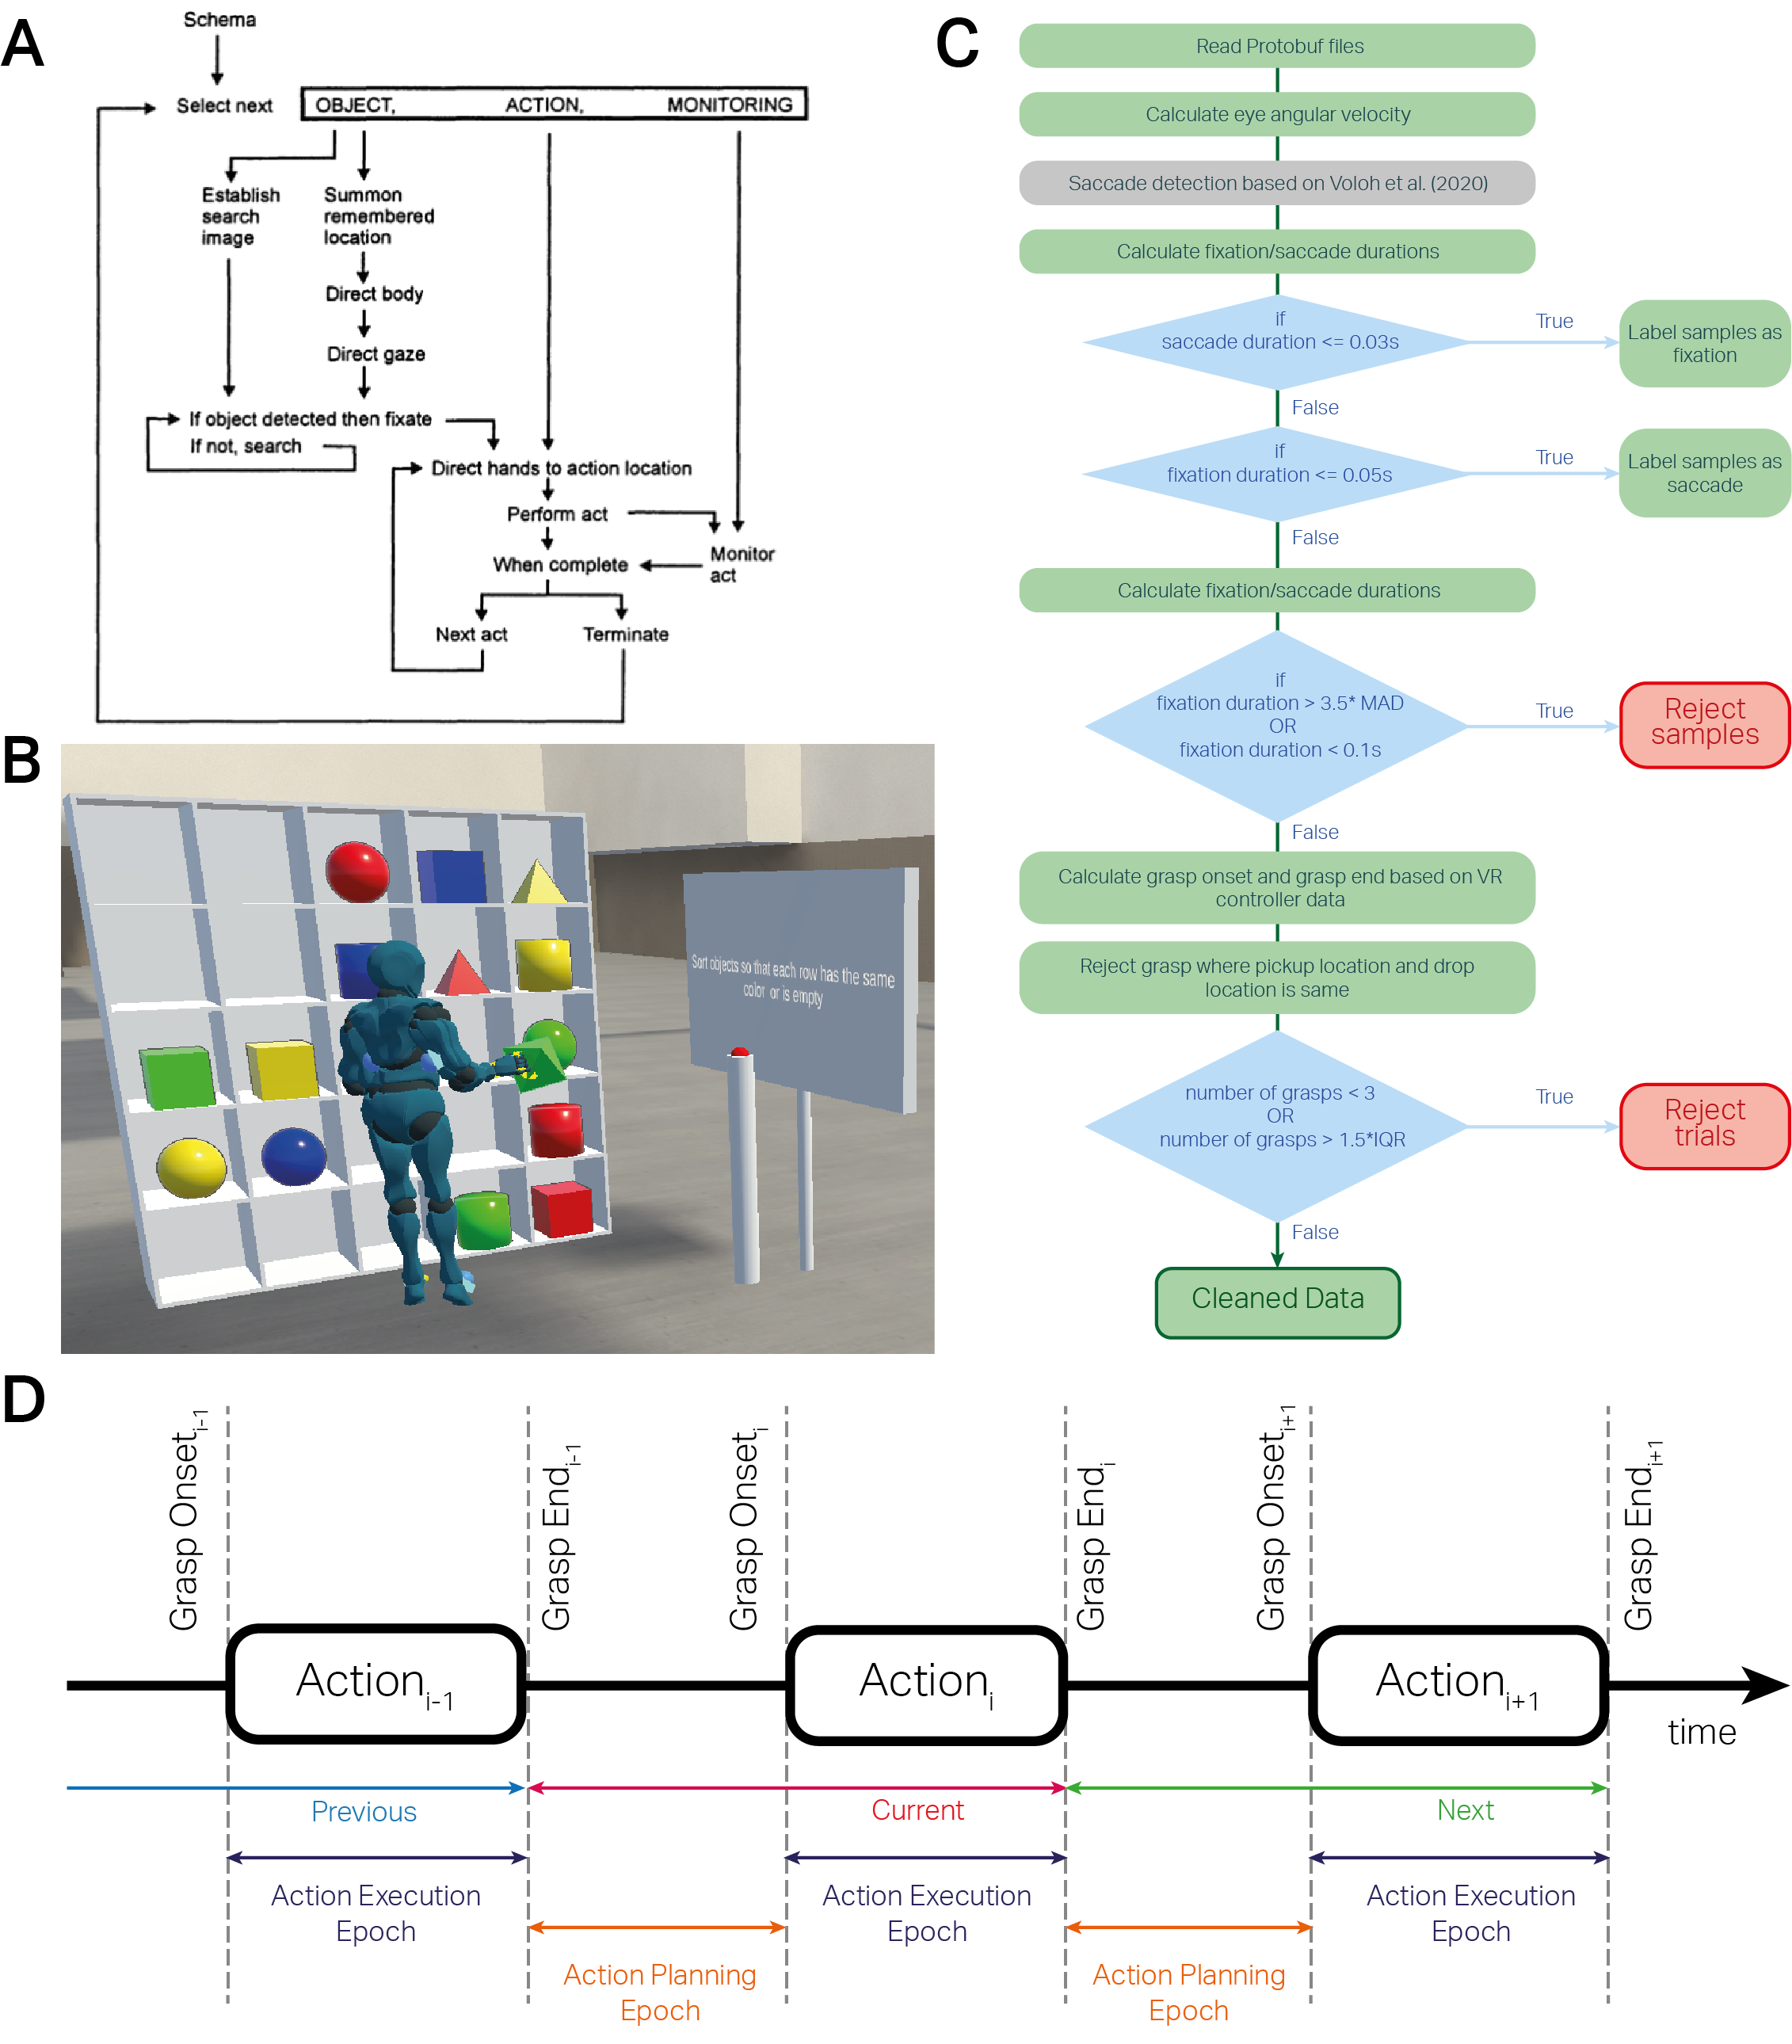
\includegraphics[width=1\linewidth]{source/figures/experiment_setup/Methods_1.png} \\
    \caption[]{\textbf{A.} Schematic of motor and gaze control during performance of natural tasks \citet{Land2001-do}. \textbf{B.} Experimental Task. In a virtual environment participants sorted 16 different objects based on 2 features color or shape while we measured their eye and body movements. The objects were randomly presented on a 5x5 shelf at the beginning of each trial and were cued to sort objects by shape and/or color. Trials where objects were sorted based on just one object feature (color or shape) were categorized as EASY trials. Conversely, in the trials where sorting was based on both features (color and shape) were categorized as HARD trials. All participants performed 24 trials in total (16 easy trials and 8 hard trials) with no time limit. \textbf{C.} Data preprocessing steps for fixation/saccade detection and data rejection. \textbf{D.} Action execution and planning epochs. In order to study the function of eye movements we divided each trial into action planning and action execution epochs. The action execution epochs start from grasp onset till grasp end for each object displacement, whereas the action planning epochs start from grasp end of previous object displacement and grasp onset of current object displacement.}
    \label{figure:task}
\end{figure}



The experimental setup consisted of 16 different objects placed on a shelf of 5x5 grid. The objects were differentiated based on two features: color and shape. We used four high contrast colors (red, blue, green and yellow) and four 3D shapes (cube, sphere, pyramid and cylinder). The objects had an average height of 20cm and width of 20cm. The shelf was designed with a height and width of 2m with 5 rows and columns of equal height, width and, depth. Participants were presented with a display board on the right side of the shelf where the trial instructions were displayed. Subjects were also presented with a red buzzer that they could use to end the trial once they finished the task. 



\subsection{Experimental Task}
Subjects performed two practice trials where they familiarized themselves with handling the VR controller and the general aspects of the setup. In these practice trials they were free to explore the virtual environment and handle the objects. After the practice trials, subjects were asked to sort object based on the one and/or two features of the object. There were two types of trials: EASY and HARD. Subjects were not limited by time to complete the task. Each subject performed 24 trials with each trial type (as listed below) randomly presented twice throughout the experiment. 
The EASY trials instructions were as follows:
\begin{enumerate}
    \item Sort objects so that each row has the same shape or is empty
    \item Sort objects so that each row has all unique shapes or is empty
    \item Sort objects so that each row has the same color or is empty
    \item Sort objects so that each row has all unique colors or is empty
    \item Sort objects so that each column has the same shape or is empty
    \item Sort objects so that each column has all unique shapes or is empty
    \item Sort objects so that each column has the same color or is empty
    \item Sort objects so that each column has all unique colors or is empty
\end{enumerate}
The HARD trials instructions were as follows:
\begin{enumerate}
    \item Sort objects so that each row has all the unique colors and all the unique shapes once
    \item Sort objects so that each column has all the unique colors and all the unique  shapes once
    \item Sort objects so that each row and column has each of the four colors once. 
    \item Sort objects so that each row and column has each of the four shapes once. 
\end{enumerate}


\subsection{Data pre-processing}

\subsubsection{Gaze Data}

The data preprocessing steps are illustrated in \ref{fig:task}C. As a first step, using eye-in-head 3d gaze direction vector for the cyclopean eye we calculated the gaze angles for the horizontal $\theta\textsubscript{h}$ and vertical $\theta\textsubscript{v}$ directions. All of the gaze data was sorted by the timestamps of the collected gaze samples. The 3d gaze direction vector of each sample is represented in $(x, y, z)$ coordinates as a unit vector that defines the direction of the gaze in VR world space coordinates. In our setup, the x coordinate corresponds to the left-right direction, y in the up-down direction, z in the forward-backward direction. The formulas used for computing the gaze angles are as follows:

 \begin{equation}\label{eq:h_angle}
     \theta\textsubscript{h} = \frac{180}{\pi} * \arctan{\frac{x}{z}}
 \end{equation}   
  \begin{equation}\label{eq:v_angle}
     \theta\textsubscript{v} = \frac{180}{\pi} * \arctan{\frac{y}{z}} 
 \end{equation}   
 
Next, we calculated the angular velocity of the eye in both the horizontal and vertical coordinates by taking a first difference of the angular velocity and dividing by the difference between the timestamp of the samples using the formula below:
\begin{equation}\label{eq:h_vel_angle}
    \omega\textsubscript{h} = \Delta\theta\textsubscript{h} / \Delta t
 \end{equation}  
 \begin{equation}\label{eq:v_vel_angle}
     \omega\textsubscript{v} = \Delta\theta\textsubscript{v} / \Delta t
 \end{equation}  

Finally, we calculated the magnitude of the angular velocity ($\omega$) at every timestamp from the horizontal and vertical components using:
\begin{equation}\label{eq:vel_angle}
     \omega = \sqrt{\omega_h^2 + \omega_v^2}
 \end{equation}  

To filter the samples where gaze was relatively stable, we used an adaptive threshold method for saccade detection described by \citet{Voloh2019-oc}. We selected an initial saccade velocity threshold $\theta\textsubscript{0}$ of 200 $\circ$/sec. All eye movement samples with an angular velocity of less than $\theta\textsubscript{0}$ were used to compute a new threshold $\theta\textsubscript{1}$. $\theta\textsubscript{1}$ was three times the median absolute deviation of the selected samples. If the difference between $\theta\textsubscript{1}$ and $\theta\textsubscript{0}$ was less than 1 $\circ$/sec $\theta\textsubscript{1}$ was selected as the saccade threshold else, $\theta\textsubscript{1}$ was used as the new saccade threshold and the above process was repeated. This was done until the difference between $\theta\textsubscript{n}$ and $\theta\textsubscript{n+1}$ was less than or equal to 1 $\circ$/sec. This way we arrived at the cluster of samples that belonged to fixations and the rest were classified as saccades. After this, we calculated the duration of the fixations and saccades. To handle miniscule fixations and saccades, we labeled all samples with saccade duration less than 0.03 seconds as a fixation. We also labeled all fixation samples with duration of less than 0.05 seconds as saccades. Following this, we recalculated the fixation and saccade durations. Finally, we rejected all fixations with duration greater than 3.5 times the median absolute deviation of the population fixation duration as well as fixations that were less than 0.1 seconds long. 


\subsubsection{Grasp data}

Subjects used the trigger button of the HTC vive controller to virtually grasp the objects on the shelf and displace them to other locations. In the data, the trigger was recorded as a boolean which was set to TRUE when a grasp was initiated and was reset to FALSE when the grasp ended. Using the position of the controller in the world space, we determined the locations from the shelf where a grasp was initiated and ended. We also removed trials where the controller data was showed implausible locations in the world space. These faulty data can be attributed to loss of tracking during the experiment. Next, we removed grasping periods where the beginning and final locations of the objects on the shelf were the same. We calculated the inter-quartile range (IQR) of the participants object displacement behavior for the two trial types (EASY and HARD). To remove the outlying object displacements in the trials, we removed the trials with 1.5 times the IQR of object displacements. We also removed those trials with fewer than three object displacements. 

\subsection{Data Analysis}\label{sec:data_analysis}

In order to study the function of eye movements for both action planning and execution, we divided each trial into 2 types of epochs. The action execution epoch spanned the time from start of object displacement to the end. The action planning epochs started from end of previous object displacement to start of current object displacement. The schematic of this epoch creation is illustrated in figure \ref{figure:task}D. This division of time within each trial into separate epochs allows us to parse the role of overt eye movements in planning and execution of object related actions separately.

For the action planning and execution epochs, we examined the spatial and temporal characteristics of eye movements while performing the sorting tasks. We divided the object and shelf locations into 7 regions-of-interest (ROIs) comprising of previous, current, and next target object and target shelf. More specifically, the previous target object refers to the object that was handled in the previous action epoch, and previous target shelf as the shelf where the previous target object was placed. Similarly, the current target object refers to the object that is picked up and placed on the target shelf in the current epoch and the next target object and next target shelf in the immediately following epoch. All other regions which did not conform to the above 6 ROIs are categorized as 'other' and not relevant to the action sequence.  As we need at least 3 object related actions within a trial to form the ROIs for the action planning and action execution epochs, we removed trials where subjects made fewer than three object displacements. In this format, we could parse the sequence of eye movements on the seven ROIs that are relevant for planning and execution of the object related actions. 


% \subsubsection{Task-based behavioral differences}\label{sec:behavior}

% In order to assess the planning behavior of the participants, we determined the optimal object displacements required to accomplish the tasks for the two trial type. To determine the optimal object displacements we designed a depth-first search algorithm that computed the minimum number of displacements required to sort the objects for the 5000 random initial configurations of 16 objects in 25 shelf locations for both EASY and HARD trial constraints. We compared the mean number of object displacements made by the participants in the EASY and HARD trials with the model based object displacements using independent t-tests.

% Next, we tested the differences in the duration of 
\subsubsection{Action Locked Gaze Control}\label{sec:avg_fixations}

We were interested in the average fixation behavior time-locked to action initiation. For each grasp onset in a trial we chose the time period from 2 seconds before grasp onset and 2 seconds after. We divided this 4 second period into bins of 0.15 seconds and calculated the number of fixations on the seven ROIs described above. For each time bin, we calculated the proportion of fixations on the ROIs per trial type (EASY, HARD). To find the time-points where there were significant differences between EASY and HARD trials for a given ROI, we used the cluster permutation method. Here, we use the t-statistic as a test statistic for each time-bin, where t is defined as:

\begin{gather*}\label{eq:cluster_permutation}
 t = \sqrt{N} * \frac{x}{\sigma}
 \end{gather*}

and, x is the mean difference between the trial types, and $\sigma$ is the standard deviation of the mean and N is the number of subjects. We used a threshold for t at 2.14 which corresponds to the t-value at which the p-value is 0.05 in the t-distribution. We first found the time-bins where the t-value was greater than the threshold. Then, we computed the sum of the t-values for these clustered time-bins which gave a single value that represented the mass of the cluster. Next, to assess the significance of the cluster, we permuted all the time-bins across trials and subjects and computed the t-values and cluster mass for 1000 different permutations. This gave us the null distribution over which we compared the cluster mass shown by the real data. To account for the multiple independent comparisons for the seven ROIs, we considered the significant clusters to have a Bonferroni corrected p-value less than 0.007 (0.05/7). In the results, we report the range of the significant time-bins for the seven ROIs for the two trial types the corresponding p-values. 

\subsubsection{Spatio-temporal Gaze Control in Action Planning and Execution}\label{sec:transitions}

To compute the scan paths within the action planning and execution epochs we created transition matrices that show the origin and destination locations of the fixations on the 7 ROIs. We used the steps described by \citet{Hooge2013-bk} to first create the scan paths and then the transition matrices. We calculated the transition matrices summarizing gaze transitions from and to the 7 ROIs from the action planning and execution epochs for each object displacement. Using the transition matrices, we calculated the net and total transitions from and to each ROI. For every transition matrix 'A' per trial, net and total transition are defined as follows:
\begin{equation}\label{eq:net_transitions}
     A_{net} = A - A^T
\end{equation}  
\begin{equation}\label{eq:total_transitions}
     A_{total} = A + A^T
\end{equation}  

As discussed in \citet{Hooge2013-bk}, if subjects make equal number of transitions between all ROIs, we can expect no transitions in the net transition matrix and can surmise that the gaze was allocated more randomly. Conversely, with strong gaze guidance we would expect more net transitions. Hence, using the net and total transitions per trial, we then calculated the relative net transitions as:

\begin{equation}\label{eq:f_value}
     Relative_{Transitions} = \frac{\sum A_{net}}{\sum A_{total}}
\end{equation}  

We then took the mean of the relative transitions per trial as a measure of gaze guidance in that trial. Higher mean relative transitions would indicate gaze allocated to ROIs in a systematic manner whereas, relative transitions would represent a random gaze allocation towards the ROIs.

Further, we also calculated the time required to first fixation on the 7 ROIs in a given planning or execution epoch. We then took the median time to first fixation per trial that would indicate time to first fixate on the ROIs for 50\% of the action planning and action execution epochs. This method was used by \citet{Montfoort2007-oa} and further applied by \citet{Hooge2013-bk} to capture the gaze attraction power of ROIs. As the action planning and execution epochs varied in duration, we normalized the time points by dividing them by the duration of the epoch. This way, time elapsed since start of an epoch is comparable to all epochs across trials and subjects.


\subsubsection{Linear Mixed Effects Models} \label{sec:lmm}
We modelled the linear relationship of the relative net transitions dependent on trial type (EASY, HARD), epoch type (planning, execution) and number of object displacements and their interactions. All within-subject effects were modeled with random intercept and slopes grouped by subject. The categorical variables trial type and epoch type were effect coded \citep{Schad2018-av}, so that the model coefficients could be interpreted as main effects. The object displacement variable which pertained to the number of object displacements in the trial were coded as a continuous numeric variable and centered on zero mean. The model fit was performed using restricted maximum likelihood (REML) estimation \citep{Corbeil1976-qq} using the lme4 package (v1.1-26) in R 3.6.1. We used the L-BFGS-B optimizer to find the best fit using 20000 iterations. Using the Satterthwaite method \citep{Luke2017-pz}, we approximated degrees of freedom of the fixed effects. The full model in Wilkinson notation \citep{Wilkinson1973-ex}  is defined as:

\begin{gather}\label{eq:lmm_formula1}
     Relative_{Transitions} \sim 1 + trial\_type * epoch\_type * object\_displacements \\
     + (1 + trial\_type * epoch\_type * object\_displacements | Subject ) 
\end{gather} 


We modelled the linear relationship of the median time to first fixation dependent on trial type (EASY, HARD) and the 7 ROIs and their interactions. We computed two models for the action planning and execution epochs as the. All within-subject effects were modeled with random intercept and slopes grouped by subject. The categorical variables trial\_type and ROI were effect coded, so that the model coefficients could be interpreted as main effects. For both models, we chose the latency of the first fixation on current target object as the reference factor so that the latency of the first fixation of all other ROIs could be compared to it. The model fit was performed using restricted maximum likelihood (REML) estimation \citep{Corbeil1976-qq} using the lme4 package (v1.1-26) in R 3.6.1. We used the L-BFGS-B optimizer to find the best fit using 20000 iterations. Using the Satterthwaite method \citep{Luke2017-pz}, we approximated degrees of freedom of the fixed effects. The full model in Wilkinson notation \citep{Wilkinson1973-ex}  is defined as:

\begin{gather}\label{eq:lmm_formula2}
     Fixation_{time} \sim 1 + trial\_type * ROI \\
     + (1 + trial\_type * ROI | Subject ) 
\end{gather} 



